\subsection{Horseshoe, Cauchy and Their Generalization}
As a continuous shrinkage prior, horseshoe prior one of the most popular local-global prior to reach the purpose of locally adaptive shrinkage because of its sharp asymptotic at the origin as well as its heavy tail. 
The density function horseshoe prior can be presented as a mixture of Gaussian distributions:
\begin{align}
    \theta_i|\nu_w^2,\tau_i^2 \sim  N(0,\nu_w^2\tau_i^2)\\
    \tau_i \sim  \pi_\tau \equiv C^+(0,1)
\end{align}
$\pi_\tau$ here is a half-Cauchy distribution for standard debiation $\tau$
To fit horseshoe priors, we choose to construct heavy tails of the local shrinkage prior by transform a Normal distribution to a heavy tail distribution through an exponential function, and then calculate activation function that can make the transformed priors approximate the horseshoe prior.
\begin{align}
    T(t)=exp(\lambda_1 sign(t)t^2), \lambda \in (0,1)
\end{align}
    For $U=T(Z)$ and $Z\sim N(0,1)$, then the density function of $U$ would be:
    \begin{align}
        f_U(u) \propto u^{-1-\frac{sing(log(u)}{2}}|log(u)|^\frac{1}{2}
    \end{align}
    This exponential activation function $T(t)$ construct a polynomial -tailed prior on $\theta\sim T(\alpha)\omega$, which align with our purpose. Figure 2 show the density of $T(\alpha)\omega$ along with $\theta$, which is almost same with the original horseshoe prior distribution.
    \begin{figure}[t]
     \centering
     \begin{subfigure}[b]{0.49\textwidth}
         \centering
         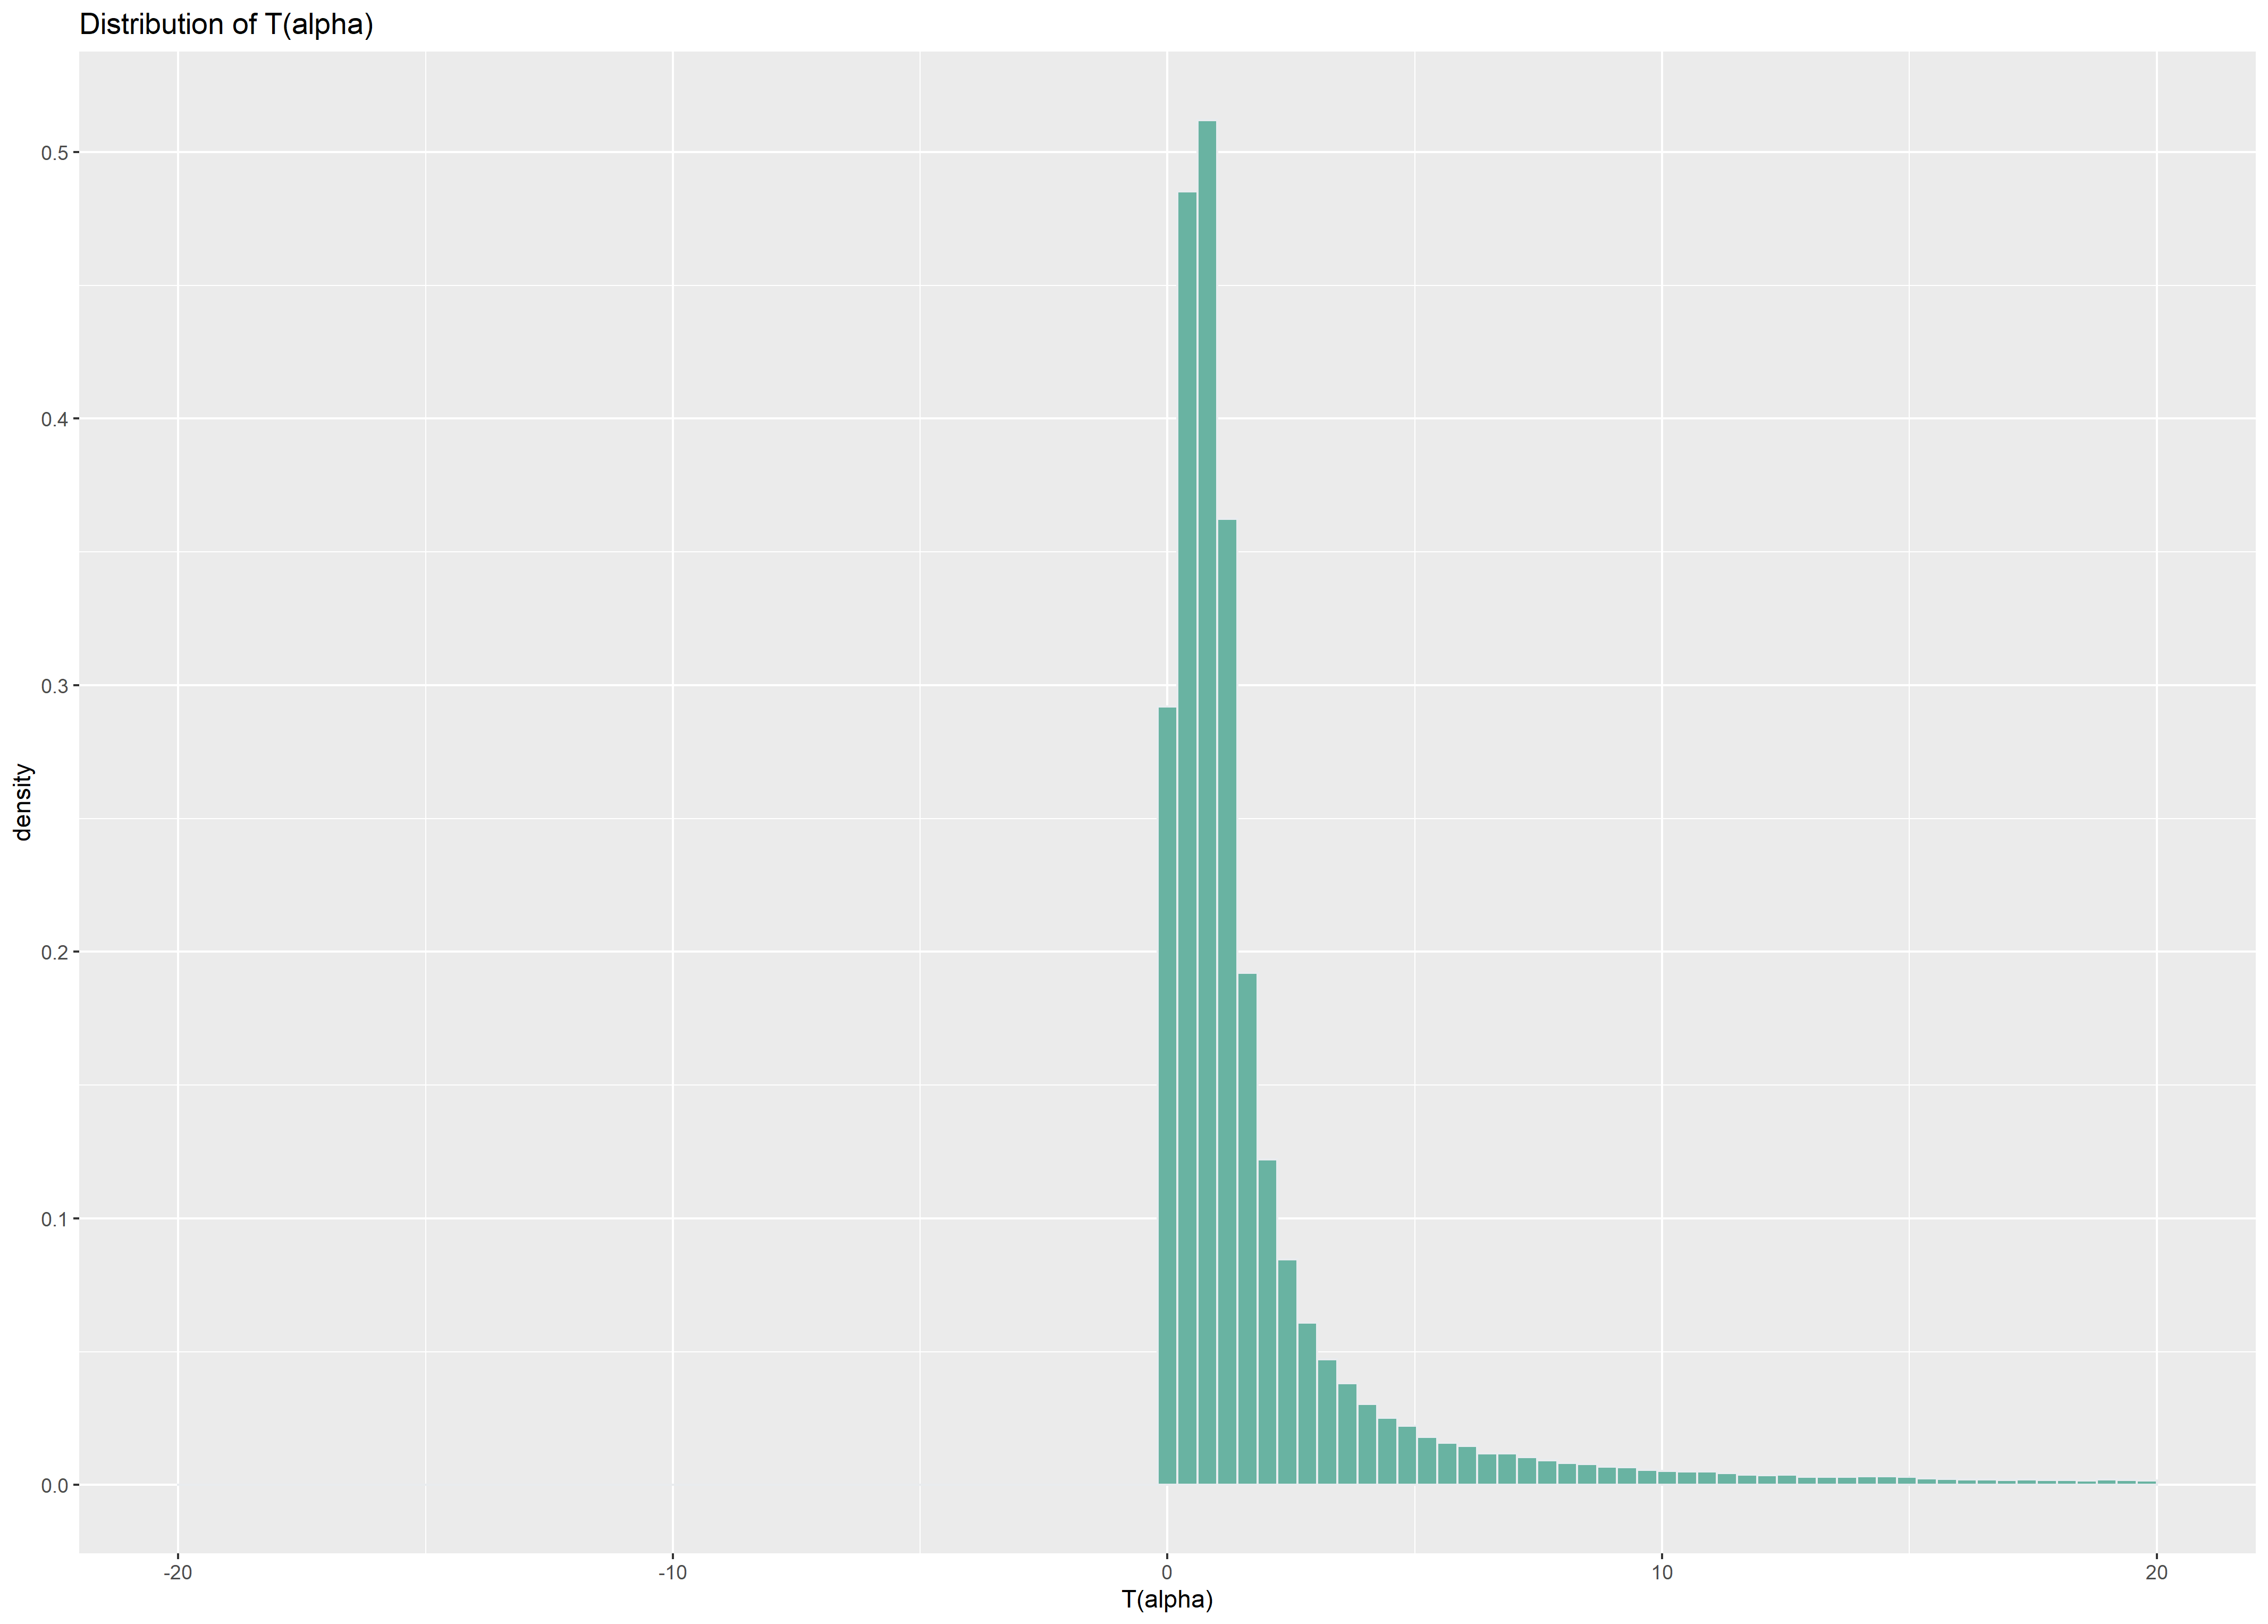
\includegraphics[width=\textwidth]{Figures/HSprior1.png}
     \end{subfigure}
     \hfill
     \begin{subfigure}[b]{0.49\textwidth}
         \centering
         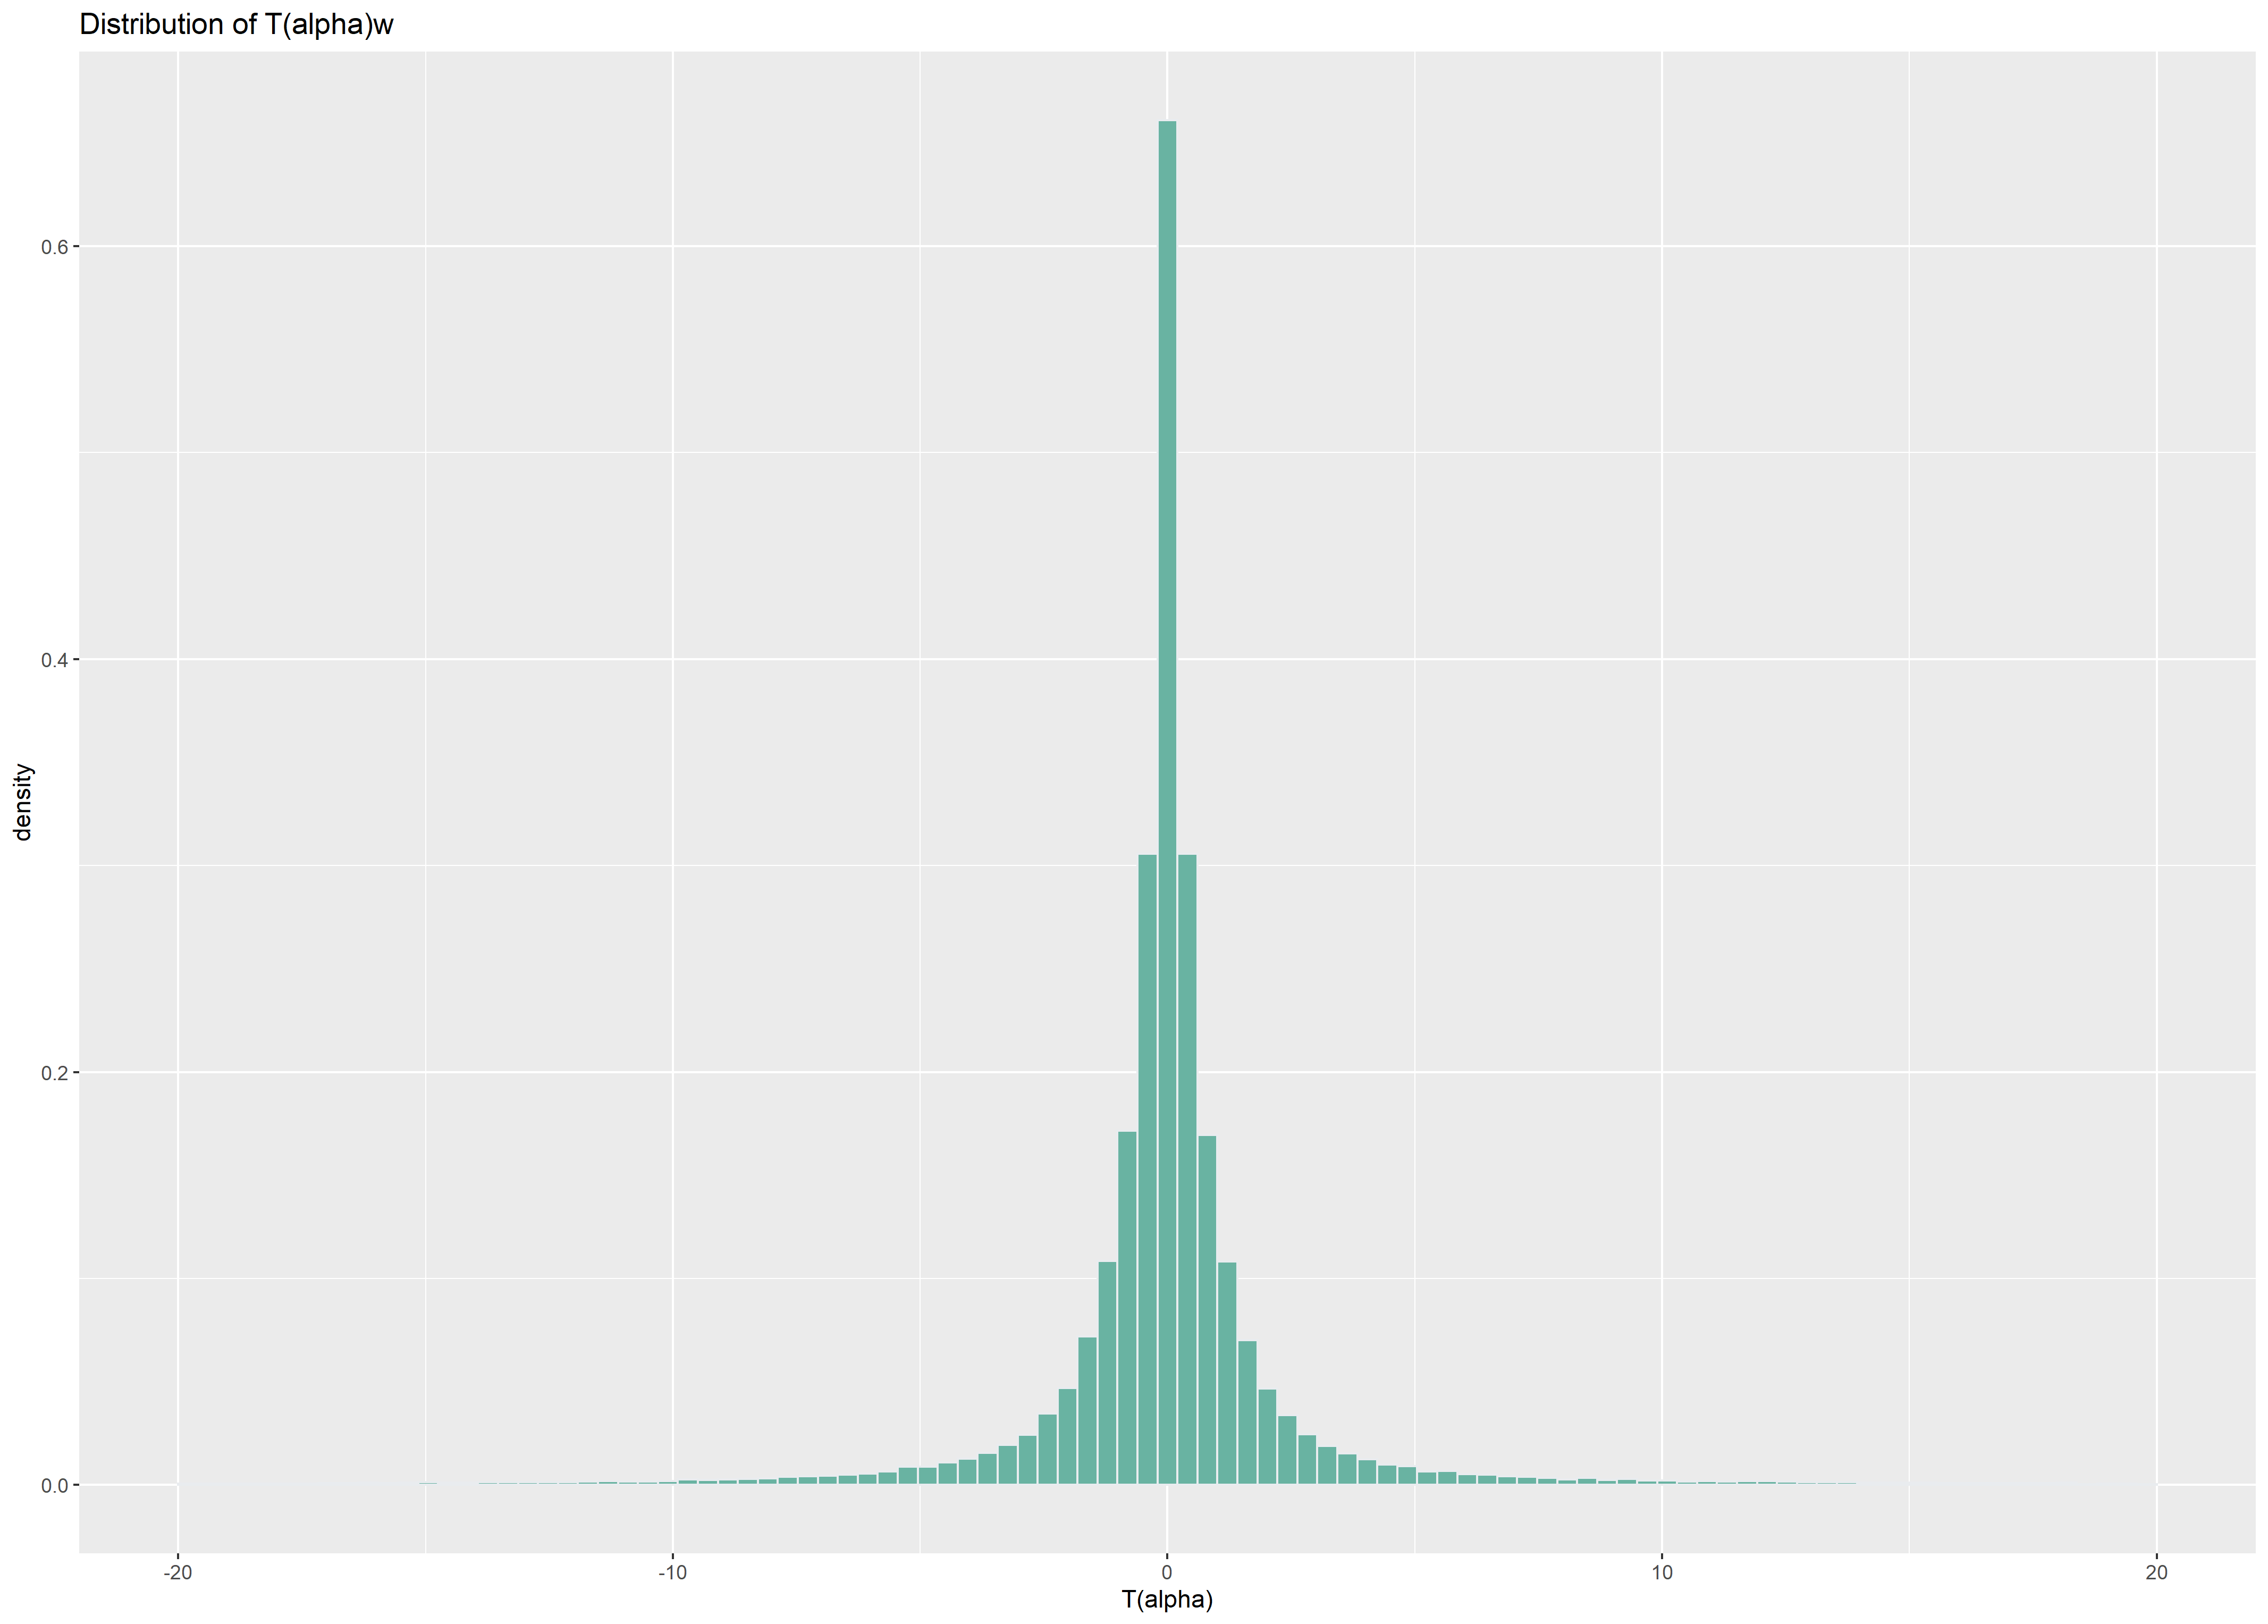
\includegraphics[width=\textwidth]{Figures/HSprior2.png}
     \end{subfigure}
     \hfill
     \begin{subfigure}[b]{0.49\textwidth}
         \centering
         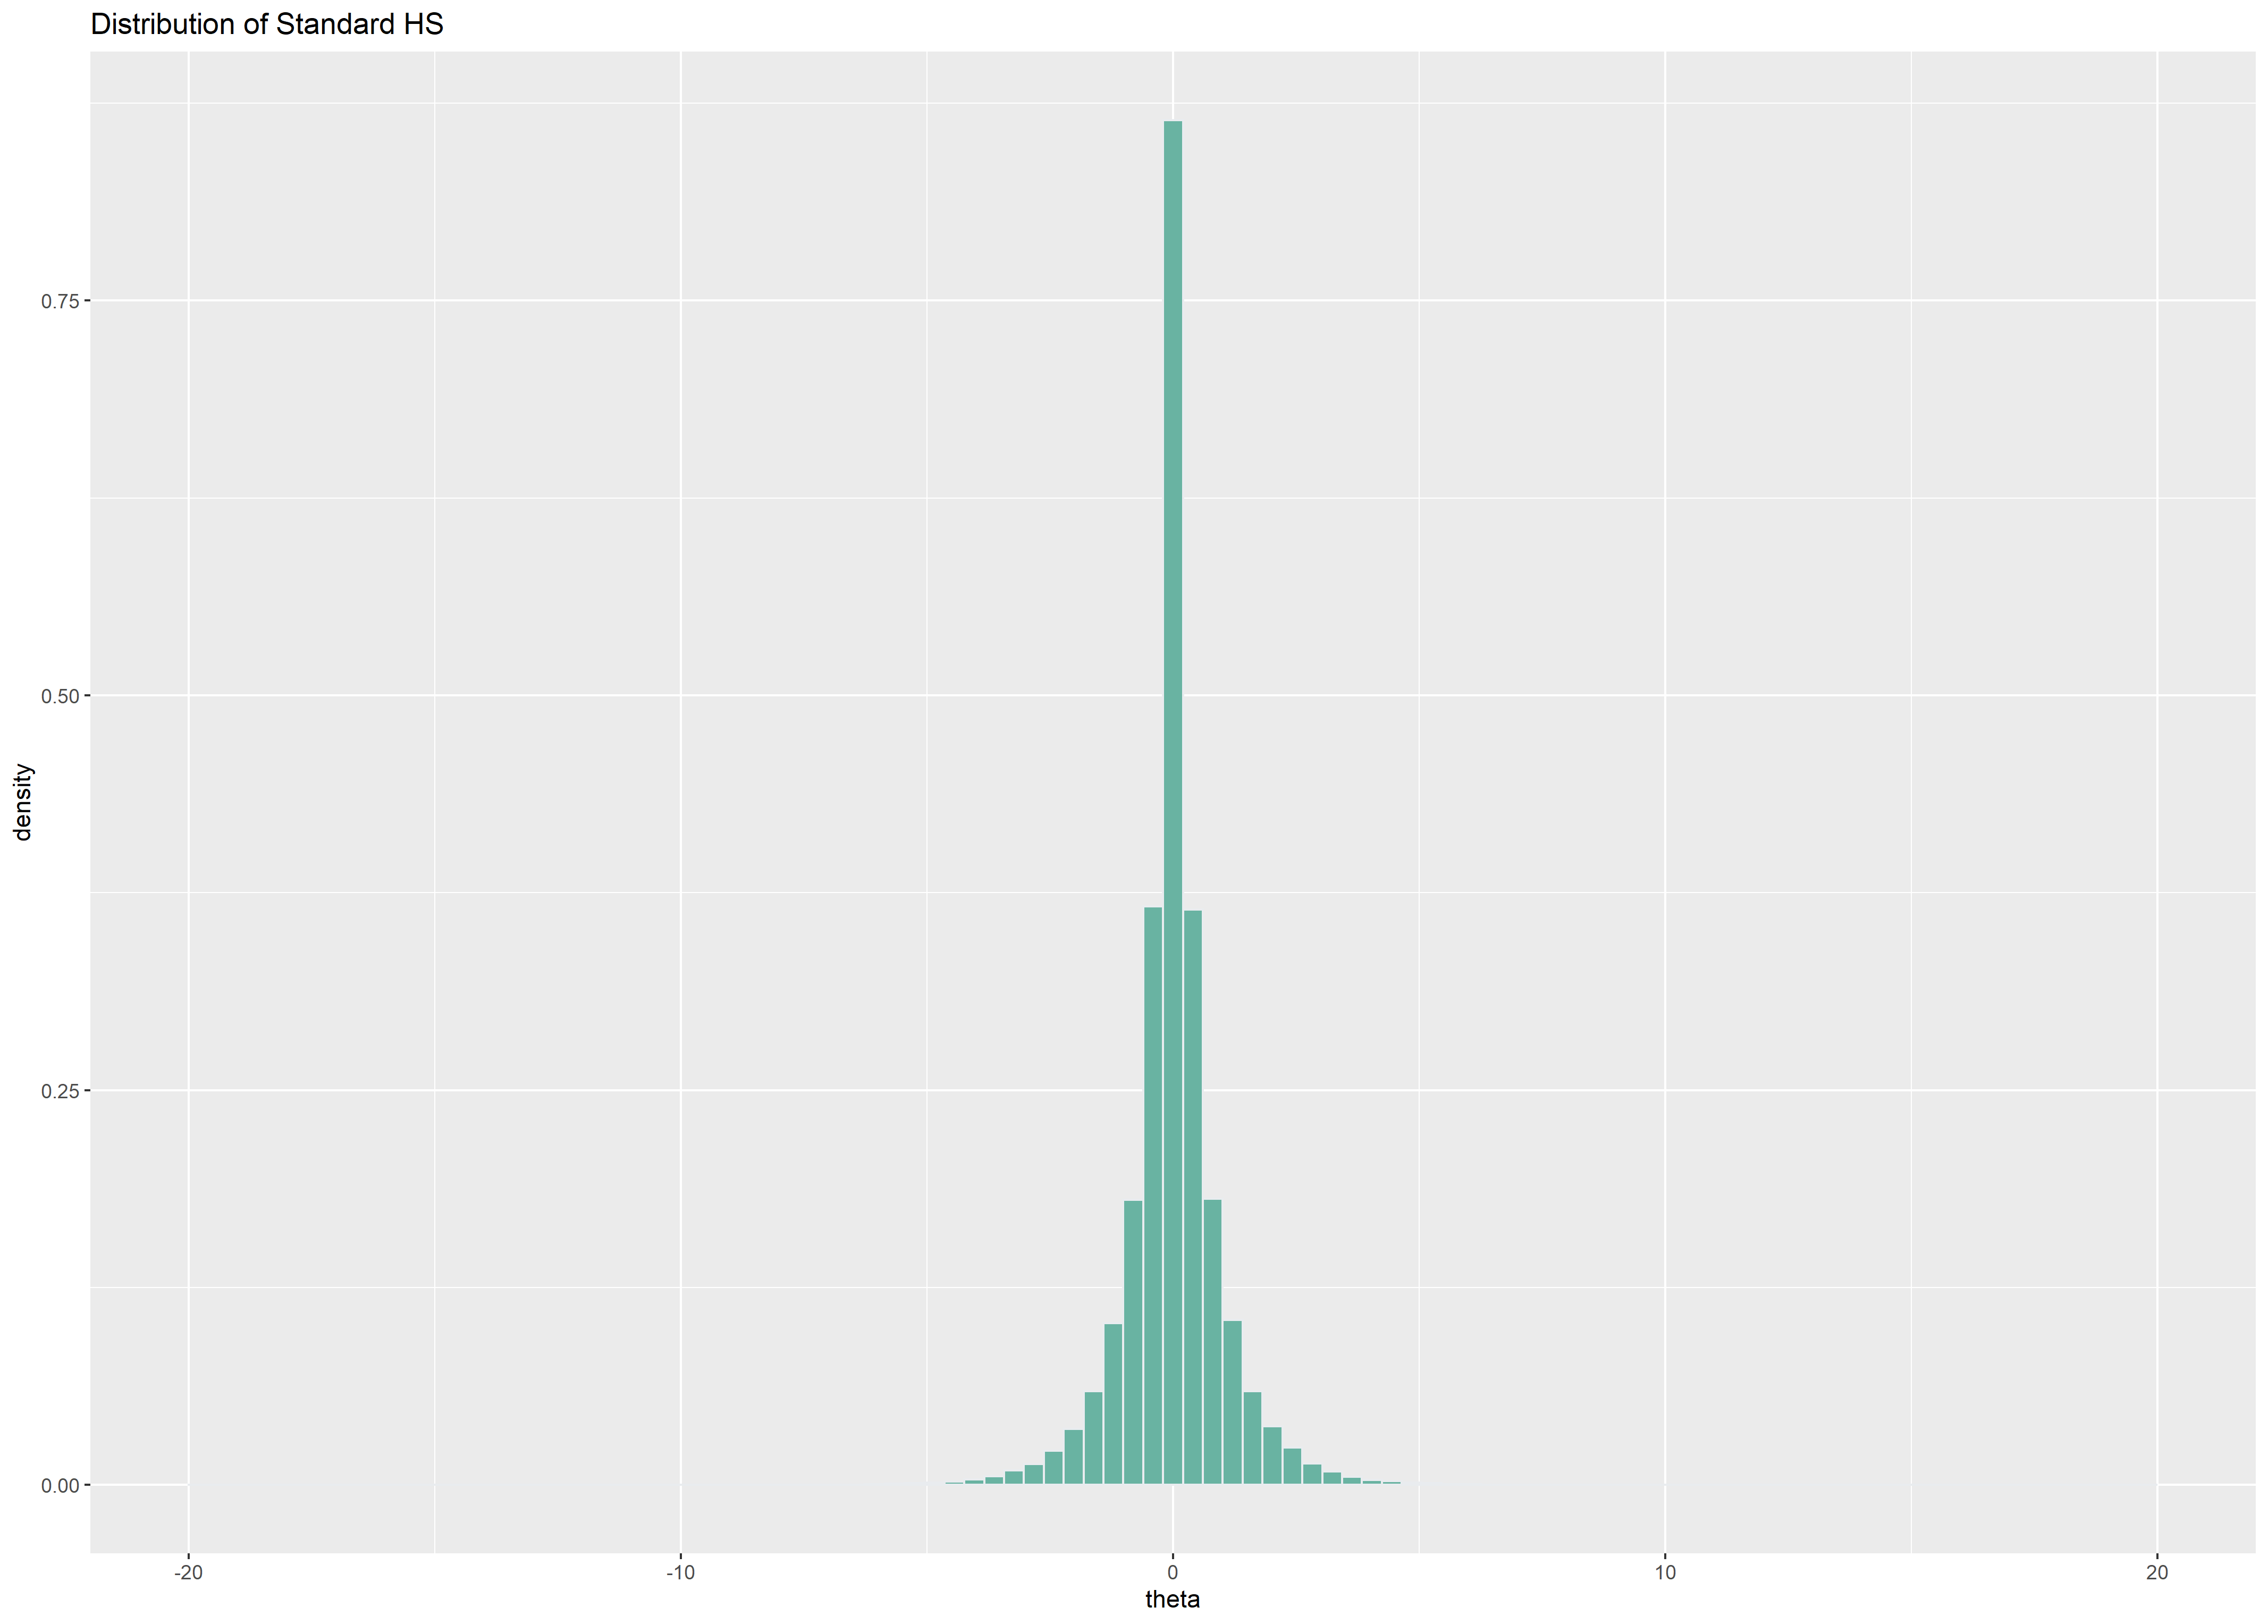
\includegraphics[width=\textwidth]{Figures/HSprior3.png}
     \end{subfigure}
        \caption{Histogram of $T(\alpha)$, $T(\alpha)w$, and the standard Horseshoe prior.}
        \label{fig:HS_prior}
\end{figure}

    In order to generalize horseshoe priors, as $\lambda_1$ indicates the tail behavior of the current neuronized prior, we add two more polynomial terms with lower exponents to the exponential activation function:
    \begin{align}
        T(t)=exp(\lambda_1 sign(t)t^2+\lambda_2 t+\lambda_3)
    \end{align}
    By numerically calculation, when $T(t)=exp(0.5 sign(t)t^2+0.733 t$, the neuronized prior approximate horseshoe prior well and $T(t)=exp(0.5 t^2-1.27t+0.29)$ approximate to standard Cauchy priors\cite{shin2021neuronized}. However, the generalized activation function for Cauchy will change to $T(t)=exp(\lambda_1 t^2+\lambda_2 t+\lambda_3)$ since this activation function will have stronger shrinkage effects for weak signals.
    
    Under this circumstance, the activation function solve the challenge that the corresponding MCMC algorithm can't achieve to geometric ergodicity under horseshoe prior, which is a heavy tail prior\cite{k1996the}. The MCMC procedure can achieve convergence more efficiently with the activation function, because the tail is stable in this case. 
   
